\documentclass[UTF8,a4paper,12pt]{ctexart}
\usepackage{geometry}
\usepackage{amsmath,amssymb}
\usepackage{booktabs}
\usepackage{array}
\usepackage{longtable}
\usepackage{multirow}
\usepackage{xcolor}
\usepackage{hyperref}
\usepackage{xurl}
\usepackage{listings}
\usepackage{enumitem}
\usepackage{graphicx}

\geometry{left=2.5cm,right=2.5cm,top=2.6cm,bottom=2.6cm}
\hypersetup{colorlinks=true,linkcolor=blue,citecolor=blue,urlcolor=blue}
\setlist{nosep}

\lstset{
  basicstyle=\ttfamily\small,
  breaklines=true,
  frame=single,
  columns=fullflexible,
  keywordstyle=\color{blue!70!black},
  commentstyle=\color{green!40!black},
  stringstyle=\color{orange!60!black}
}

\title{\textbf{基于动态知识图谱注意力的餐饮外卖个性化推荐}}
\author{推荐系统/大数据课程作业}
\date{\today}

\begin{document}
\maketitle

\begin{abstract}
餐饮外卖推荐具有明显的时效性和场景性：同一用户在早餐、午餐、晚餐或不同日期可能表现出不同饮食偏好，且用户下单前的点击序列往往暴露了短期意图。本文构建一个不依赖骑手和配送数据的餐饮外卖商家推荐模型，使用公开的美团外卖 TRD 数据集，融合用户历史订单、商家属性、餐饮知识图谱、时间衰减和点击序列生成的临时兴趣节点。模型将用户连续行为序列转化为动态图谱上的带权边，而不是采用传统序列推荐结构；在动态图谱上使用关系感知注意力机制聚合用户当前兴趣表示，并将该表示、候选商家图谱表示与基础特征输入排序层，输出 Top-K 商家推荐及基于图谱路径的解释。实验在真实 TRD 的 10 万订单子集上完成，每个测试请求包含 1 个真实下单商家和 199 个负候选商家。结果显示，最终融合模型在 Recall@5、Recall@10、Recall@20、NDCG@10、MRR 和 AUC 上均取得本实验最佳结果，说明协同过滤邻域信号与动态图谱短期兴趣信号具有互补性。
\end{abstract}

\noindent\textbf{关键词：} 外卖推荐；动态知识图谱；时间衰减；临时兴趣节点；关系感知注意力；可解释推荐

\section{课题背景与目标}

餐饮外卖推荐区别于电影、图书、电商等场景，主要体现在三点。第一，饮食偏好具有较强时效性，用户昨天想吃川菜并不代表今天仍然想吃川菜。第二，外卖下单前的点击序列包含短期意图，例如用户连续浏览低价快餐、轻食或某一区域商家，往往说明当前一餐的偏好正在变化。第三，餐饮商家可通过菜系、口味、价格、评分、区域、品牌、菜品食材等知识图谱属性解释。

本文目标是构建一个不使用骑手、配送时长、配送距离等配送侧数据的 Top-K 个性化商家推荐模型。模型输入包括用户历史订单、下单前点击商家序列、商家属性和菜品属性；输出为候选商家偏好得分、Top-K 推荐列表和解释路径。

\section{数据集选择与字段需求}

\subsection{数据集}

本文选用公开数据集 TRD: Takeout Recommendation Dataset from Meituan Takeout app\cite{trd2023}。该数据集收集自美团外卖 App，覆盖北京 11 个商圈，时间范围为 2021-03-01 至 2021-03-28。官方划分中，前三周订单作为训练集，最后一周订单作为测试集，避免未来信息泄漏。数据集包含用户属性、外卖商家属性、菜品属性、订单-商家交互、订单-菜品交互以及下单前点击商家序列。美团技术团队关于外卖美食知识图谱的文章也指出，外卖美食知识图谱通常包含菜品类目、标准菜品、食材、口味、菜系等标签，可服务搜索和推荐等业务\cite{meituan_kg_blog}。

本项目已下载 TRD 文本文件至 \texttt{data/raw}，没有使用体积较大的 \texttt{graph.bin}，而是从文本文件重新构造本文所需知识图谱。主要文件如下：

\begin{table}[htbp]
\centering
\caption{TRD 主要文件与字段用途}
\begin{tabular}{p{4.0cm}p{10.0cm}}
\toprule
文件 & 本文使用方式 \\
\midrule
\texttt{users.txt} & 用户 ID、历史平均消费区间、工作日/周末平均消费区间，用作用户基础特征。\\
\texttt{pois.txt} & 商家 ID、商家名称、一级/二级/三级餐饮类目、品牌、区域、商家评分、配送评分、食品评分，用于构造商家属性实体和商家基础特征。\\
\texttt{spus.txt} & 菜品 ID、菜品名、价格、菜品类目、食材、口味、标准菜品 ID，用于补充商家关联的菜品知识。\\
\texttt{orders\_train.txt} & 训练期订单-商家交互，包含用户、订单、商家、价格区间、下单时间、餐段、场景、地址区域等字段。\\
\path{orders_test_poi.txt} 与 \path{orders_poi_test_label.txt} & 测试期订单上下文与真实下单商家标签，用于 Top-K 评价。\\
\path{orders_poi_session.txt} & 每笔订单前点击过的商家序列，用于生成临时兴趣节点。\\
\path{orders_spu_train.txt} & 训练订单中的菜品，用于将菜品类目、食材、口味、标准菜品聚合到商家。\\
\bottomrule
\end{tabular}
\end{table}

字段需求可概括为：用户 ID、商家 ID、下单时间、订单价格区间、餐段、商家区域、商家评分、商家类别、菜品属性以及下单前点击序列。本文不使用骑手 ID、配送轨迹、配送时长等配送侧信息。

\section{餐饮知识图谱设计}

\subsection{实体设计}

知识图谱实体包括：

\begin{itemize}
  \item 用户实体：\texttt{user:\{user\_id\}}。
  \item 商家实体：\texttt{poi:\{wm\_poi\_id\}}。
  \item 餐饮类目实体：一级、二级、三级类目，如 \texttt{cat1:0}、\texttt{cat2:1}。
  \item 口味实体：由菜品 \texttt{taste} 字段抽取，如 \texttt{taste:1}。
  \item 食材实体：由菜品 \texttt{ingredients} 字段抽取，如 \texttt{ingredient:3}。
  \item 价格区间实体：由订单价格聚合到商家，如 \texttt{price:<29}。
  \item 评分等级实体：将评分离散为 \texttt{low}、\texttt{medium}、\texttt{high}、\texttt{excellent}。
  \item 区域实体：商家所在 \texttt{aor\_id}。
  \item 品牌实体、标准菜品实体、菜品类目实体。
  \item 临时兴趣实体：对用户当前请求动态生成，不作为全局静态实体保存，而是在样本中表示为 ``用户 $\rightarrow$ 当前偏好 $\rightarrow$ 图谱实体'' 的动态边。
\end{itemize}

\subsection{关系与三元组}

静态知识图谱三元组记为 $(h,r,t)$，其中 $h$ 多为商家实体，$t$ 为属性实体。本文构造的关系包括：

\begin{table}[htbp]
\centering
\caption{知识图谱关系设计}
\begin{tabular}{p{4.5cm}p{7.0cm}p{3.0cm}}
\toprule
关系 & 三元组示例 & 来源 \\
\midrule
\texttt{has\_cat1/2/3} & 商家 $\rightarrow$ 一级/二级/三级类目 & \texttt{pois.txt}\\
\texttt{has\_brand} & 商家 $\rightarrow$ 品牌 & \texttt{pois.txt}\\
\texttt{located\_in\_aor} & 商家 $\rightarrow$ 区域 & \texttt{pois.txt}\\
\texttt{has\_price} & 商家 $\rightarrow$ 价格区间 & 训练订单聚合\\
\texttt{has\_poi\_score} & 商家 $\rightarrow$ 商家评分等级 & \texttt{pois.txt}\\
\texttt{has\_delivery\_score} & 商家 $\rightarrow$ 配送评分等级 & \texttt{pois.txt}\\
\texttt{has\_food\_score} & 商家 $\rightarrow$ 食品评分等级 & \texttt{pois.txt}\\
\texttt{has\_food\_category} & 商家 $\rightarrow$ 菜品类目 & 订单菜品聚合\\
\texttt{has\_ingredient} & 商家 $\rightarrow$ 食材 & 订单菜品聚合\\
\texttt{has\_taste} & 商家 $\rightarrow$ 口味 & 订单菜品聚合\\
\texttt{has\_standard\_food} & 商家 $\rightarrow$ 标准菜品 & 订单菜品聚合\\
\texttt{pref\_hist} & 用户 $\rightarrow$ 历史衰减兴趣实体 & 动态构造\\
\texttt{pref\_click} & 用户 $\rightarrow$ 点击临时兴趣实体 & 动态构造\\
\bottomrule
\end{tabular}
\end{table}

在实现中，静态商家属性由 \path{src/prepare_data.py} 生成，并导出为 \path{data/processed/*.kg_triples.tsv}。本文最终实验数据包包含 243181 条静态知识图谱三元组。

\section{动态图谱构造}

\subsection{历史订单时间衰减}

设用户 $u$ 在时间 $t$ 与商家 $i$ 发生过订单交互，当前推荐请求时间为 $T$。外卖偏好具有时效性，因此历史订单边权采用指数衰减：

\begin{equation}
w_{u,i,t}=\exp(-\lambda (T-t)).
\end{equation}

其中 $T-t$ 以天为单位，$\lambda$ 控制衰减速度。本文默认 $\lambda=0.12$。若商家 $i$ 与实体 $e$ 通过静态图谱相连，记 $A_{i,e}=1$，则用户对兴趣实体 $e$ 的历史偏好为：

\begin{equation}
p^{hist}_{u,e}=\sum_{(i,t)\in \mathcal{H}_{u,T}} w_{u,i,t} A_{i,e}.
\end{equation}

这一步将用户历史订单序列转换为动态图谱上的带权兴趣边，而不是直接使用 RNN、Transformer 等传统序列推荐结构。

\subsection{临时兴趣节点}

下单前点击序列反映当前一餐的短期偏好。设订单前点击商家序列为：

\begin{equation}
\mathcal{C}_{u,T}=(c_1,c_2,\ldots,c_m).
\end{equation}

越靠近下单的点击权重越高：

\begin{equation}
w^{click}_{u,c_j,T}=\eta \rho^{m-j},
\end{equation}

其中 $\eta$ 为点击信号强度，$\rho$ 为点击衰减系数。本文默认 $\eta=1.6,\rho=0.88$。点击序列生成临时偏好：

\begin{equation}
p^{click}_{u,e}=\sum_{c_j\in \mathcal{C}_{u,T}} w^{click}_{u,c_j,T} A_{c_j,e}.
\end{equation}

最终将两类偏好边合并为动态图谱邻居集合：

\begin{equation}
\mathcal{N}^{dyn}_{u,T}=\{(e,\texttt{pref\_hist},p^{hist}_{u,e})\}\cup
\{(e,\texttt{pref\_click},p^{click}_{u,e})\}.
\end{equation}

为控制复杂度，每个用户请求保留权重最高的若干兴趣实体；该上限由
\path{max_interests} 参数控制。

\section{关系感知图注意力模型}

\subsection{用户动态兴趣聚合}

记用户 embedding 为 $\mathbf{q}_u$，兴趣实体 embedding 为 $\mathbf{e}_e$，关系 embedding 为 $\mathbf{r}$，动态偏好权重为 $p_{u,e}$。关系感知注意力分数定义为：

\begin{equation}
s_{u,e,r}=
\mathbf{a}^{\top}\tanh(W_q\mathbf{q}_u+W_e\mathbf{e}_e+W_r\mathbf{r})
\;+\;\beta\log(1+p_{u,e}).
\end{equation}

其中 $\log(1+p_{u,e})$ 将时间衰减或点击临时偏好作为 softmax 偏置，$\beta$ 在实现中吸收进模型参数和权重尺度。注意力权重为：

\begin{equation}
\alpha_{u,e,r}=
\frac{\exp(s_{u,e,r})}{\sum_{(e',r')\in \mathcal{N}^{dyn}_{u,T}}\exp(s_{u,e',r'})}.
\end{equation}

用户当前兴趣表示：

\begin{equation}
\mathbf{h}_{u,T}=
\mathrm{LayerNorm}\left(
\mathbf{q}_u+\sum_{(e,r)\in \mathcal{N}^{dyn}_{u,T}}
\alpha_{u,e,r}(\mathbf{e}_e+\mathbf{r})
\right).
\end{equation}

\subsection{候选商家表示}

候选商家 $v$ 的静态图谱邻居为 $\mathcal{N}_v$。模型对商家的类目、价格、评分、区域、食材、口味等属性也做注意力聚合：

\begin{equation}
\mathbf{g}_v=\mathrm{LayerNorm}\left(
\mathbf{v}+\sum_{(e,r)\in \mathcal{N}_v}\gamma_{v,e,r}(\mathbf{e}_e+\mathbf{r})
\right),
\end{equation}

其中 $\gamma$ 是以商家 embedding 为 query 的属性注意力。

\subsection{排序层}

最终排序层采用 MLP，将动态图谱用户表示、候选商家表示、二者逐元素乘积以及基础特征拼接：

\begin{equation}
\mathrm{score}(u,v,T)=
\mathrm{MLP}([\mathbf{h}_{u,T},\mathbf{g}_v,\mathbf{h}_{u,T}\odot \mathbf{g}_v,\mathbf{x}_{u,v,T}]).
\end{equation}

基础特征 $\mathbf{x}_{u,v,T}$ 包括用户消费区间、商家评分、商家价格、用户价格偏好与商家价格匹配度、上下文区域是否一致、餐段 one-hot 等。训练目标为二分类交叉熵，正样本为真实下单商家，负样本为从未交互商家采样。排序层也可替换为 LightGBM 或 DeepFM。DeepFM 通过结合因子分解机和深度网络建模低阶与高阶特征交互，适合作为工业 CTR 排序层参考\cite{deepfm}。

\section{实验流程}

\subsection{数据处理}

实验代码位于项目根目录。处理流程如下：

\begin{enumerate}
  \item 下载 TRD 文本文件：\texttt{python3 scripts/download\_trd.py --raw-dir data/raw}。
  \item 构建知识图谱与动态图谱样本：\texttt{python3 -m src.prepare\_data ...}。
  \item 训练 baseline 和消融模型：\texttt{python3 -m src.run\_baselines ...} 与 \texttt{python3 -m src.run\_experiment ...}。
  \item 生成解释样例：\texttt{python3 -m src.explain\_recommend ...}。
\end{enumerate}

本文最终实验使用 \texttt{trd\_gpu\_100k\_match} 数据包。该数据包由 100000 条训练订单采样得到；训练时每个正样本配 5 个负样本，因此得到 600000 个 pointwise 训练样本；每个测试请求包含 200 个候选商家，其中 1 个为真实下单商家、199 个为负候选，候选顺序在预处理阶段随机打乱：

\begin{table}[htbp]
\centering
\caption{真实 TRD 子集规模}
\begin{tabular}{lrrrrrr}
\toprule
数据包 & 用户数 & 商家数 & 实体数 & 关系数 & 训练样本 & 测试查询 \\
\midrule
\texttt{trd\_gpu\_100k\_match} & 77576 & 29071 & 5713 & 16 & 600000 & 10000\\
\bottomrule
\end{tabular}
\end{table}

该数据包在用户、商家和上下文基础特征之外，加入 6 维动态兴趣匹配特征，包括历史兴趣命中权重、点击兴趣命中权重、总命中权重及对应归一化重合比例，最终 \texttt{basic\_dim}=22。动态图谱构造默认保留最近 30 条历史订单、下单前最多 20 个点击商家和权重最高的 64 个动态兴趣实体。

\subsection{评价指标}

设推荐列表前 $K$ 个商家为 $\mathcal{R}_K(u)$，测试正样本集合为 $\mathcal{G}(u)$，本文使用：

\begin{itemize}
  \item Recall@K：$\frac{|\mathcal{R}_K(u)\cap \mathcal{G}(u)|}{|\mathcal{G}(u)|}$。
  \item Precision@K：$\frac{|\mathcal{R}_K(u)\cap \mathcal{G}(u)|}{K}$。
  \item HitRate@K：前 $K$ 是否命中至少一个正样本。
  \item NDCG@K：考虑命中位置折损的排序质量。
  \item MRR：第一个正样本排名倒数。
  \item AUC：正样本得分高于负样本的概率。
\end{itemize}

由于 TRD 测试集中每个查询只有 1 个真实下单商家，单个测试点的 Recall@K 等价于 HitRate@K，即真实商家是否进入 Top-K：命中为 1，未命中为 0。表中 Recall@K 为所有测试查询的平均命中率。例如 Recall@10=0.210 表示约 21.0\% 的测试订单中，真实下单商家被排进 200 个候选中的前 10。由于评价不是对全部 29071 个商家全排序，而是在 1 个正样本和 199 个采样负样本上排序，因此本文将其称为 sampled Recall@K。NDCG@K 和 MRR 进一步反映真实商家在 Top-K 内的具体排名位置。

\section{Baseline 与消融实验设计}

本文设置如下 baseline、动态图谱模型和最终融合模型。所有模型使用同一套 200 候选测试集，确保指标可直接比较。

\begin{itemize}
  \item Popularity：按训练集中商家下单次数排序。
  \item UserCF：基于用户历史商家集合的余弦相似用户协同过滤。
  \item ItemCF：基于商家共同用户集合的 Jaccard 相似商家协同过滤。
  \item Matrix Factorization：用户和商家 embedding 点积。
  \item 普通知识图谱推荐模型/Static KG：聚合候选商家静态图谱属性，不使用动态兴趣。
  \item KG + Time Decay：使用历史订单时间衰减兴趣边。
  \item KG + Time Decay + Temporary Interest Nodes：加入点击序列生成的临时兴趣节点。
  \item Dynamic KG Attention：Dynamic KG + Relation Attention + Ranking Layer，并加入动态兴趣匹配特征。
  \item Final Hybrid：将 ItemCF 分数与 Dynamic KG Attention 分数进行查询内标准化后线性融合。
\end{itemize}

LightGCN 是图协同过滤推荐的重要 baseline，其核心思想是去除传统 GCN 中对协同过滤贡献较小的特征变换与非线性，仅保留邻域线性传播\cite{lightgcn}。本项目在 \path{src/lightgcn.py} 中提供了 LightGCN 基础实现；报告主表使用 Static KG 作为 ``LightGCN 或普通 KG 推荐模型'' 要求中的普通 KG baseline。KGAT 则证明了知识图谱注意力网络可利用高阶连通性提升推荐准确性与解释性\cite{kgat}，本文模型在其思想基础上进一步加入外卖订单时间衰减和点击临时兴趣。

需要说明的是，Static KG、KG + Time、KG + Time + Temp 和 Dynamic KG Attention 的差异并不只在排序层，而是逐步打开动态图谱模块：Static KG 只聚合候选商家属性；KG + Time 加入用户历史订单的时间衰减兴趣；KG + Time + Temp 再加入点击序列临时兴趣；Dynamic KG Attention 在此基础上使用关系感知注意力区分 \texttt{pref\_hist}、\texttt{pref\_click} 和商家属性关系。

\section{实验结果与分析}

\begin{table}[htbp]
\centering
\caption{\texttt{trd\_gpu\_100k\_match} 上的 sampled Top-K 结果（200 候选）}
\small
\begin{tabular}{lrrrrrr}
\toprule
模型 & Recall@5 & Recall@10 & Recall@20 & NDCG@10 & MRR & AUC \\
\midrule
Popularity & 0.032 & 0.068 & 0.133 & 0.031 & 0.037 & 0.613\\
UserCF & 0.120 & 0.144 & 0.190 & 0.115 & 0.119 & 0.550\\
ItemCF & 0.135 & 0.170 & 0.223 & 0.127 & 0.128 & 0.568\\
MF & 0.117 & 0.147 & 0.204 & 0.107 & 0.110 & 0.639\\
Static KG & 0.072 & 0.120 & 0.199 & 0.065 & 0.066 & 0.654\\
KG + Time Decay & 0.050 & 0.090 & 0.168 & 0.043 & 0.048 & 0.638\\
KG + Time + Temp & 0.082 & 0.139 & 0.234 & 0.070 & 0.069 & 0.680\\
Dynamic KG Attention & 0.106 & 0.162 & 0.254 & 0.092 & 0.089 & 0.689\\
Final Hybrid & \textbf{0.157} & \textbf{0.210} & \textbf{0.294} & \textbf{0.147} & \textbf{0.146} & \textbf{0.702}\\
\bottomrule
\end{tabular}
\end{table}

\begin{figure}[htbp]
\centering
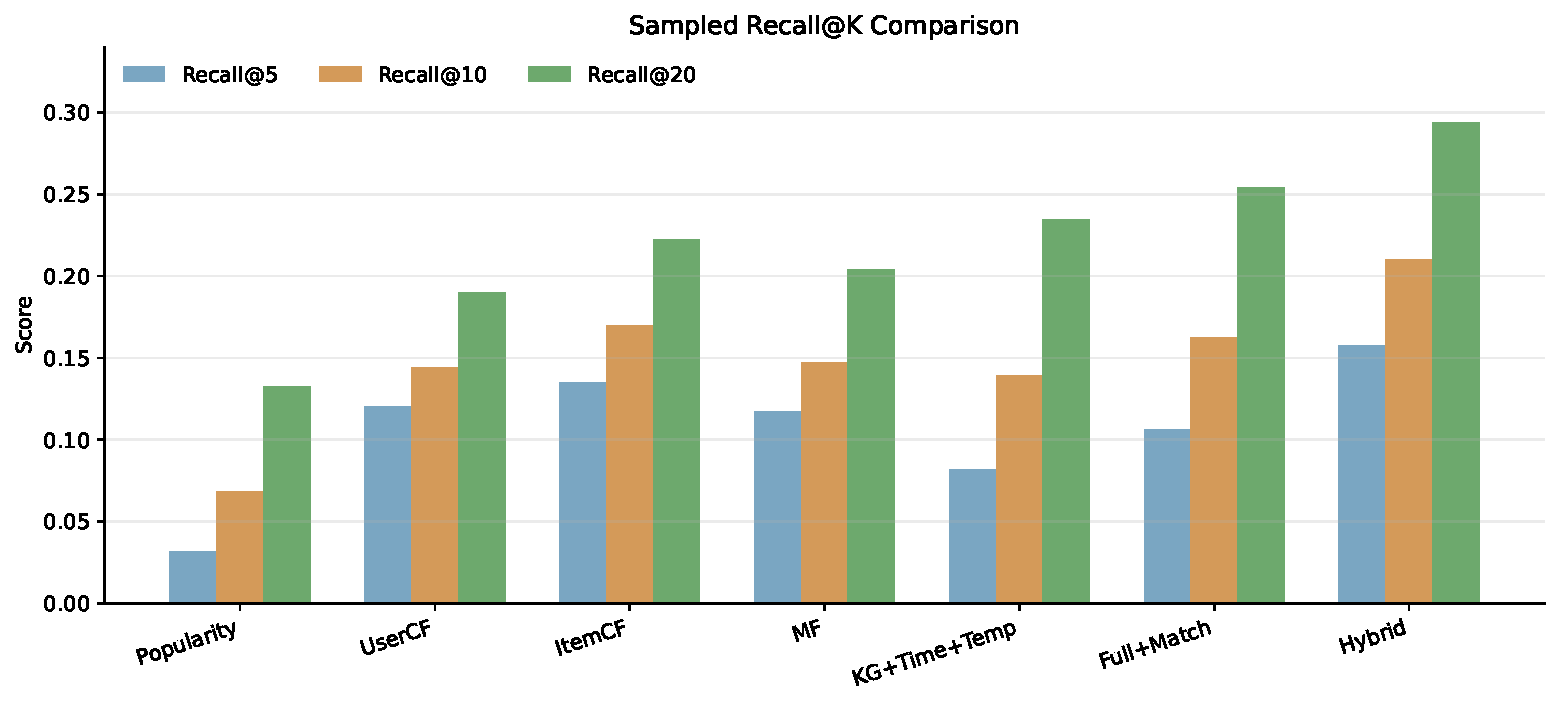
\includegraphics[width=0.96\linewidth]{figures/recall_comparison.pdf}
\caption{主要模型在 Recall@5、Recall@10、Recall@20 上的对比}
\end{figure}

\begin{figure}[htbp]
\centering
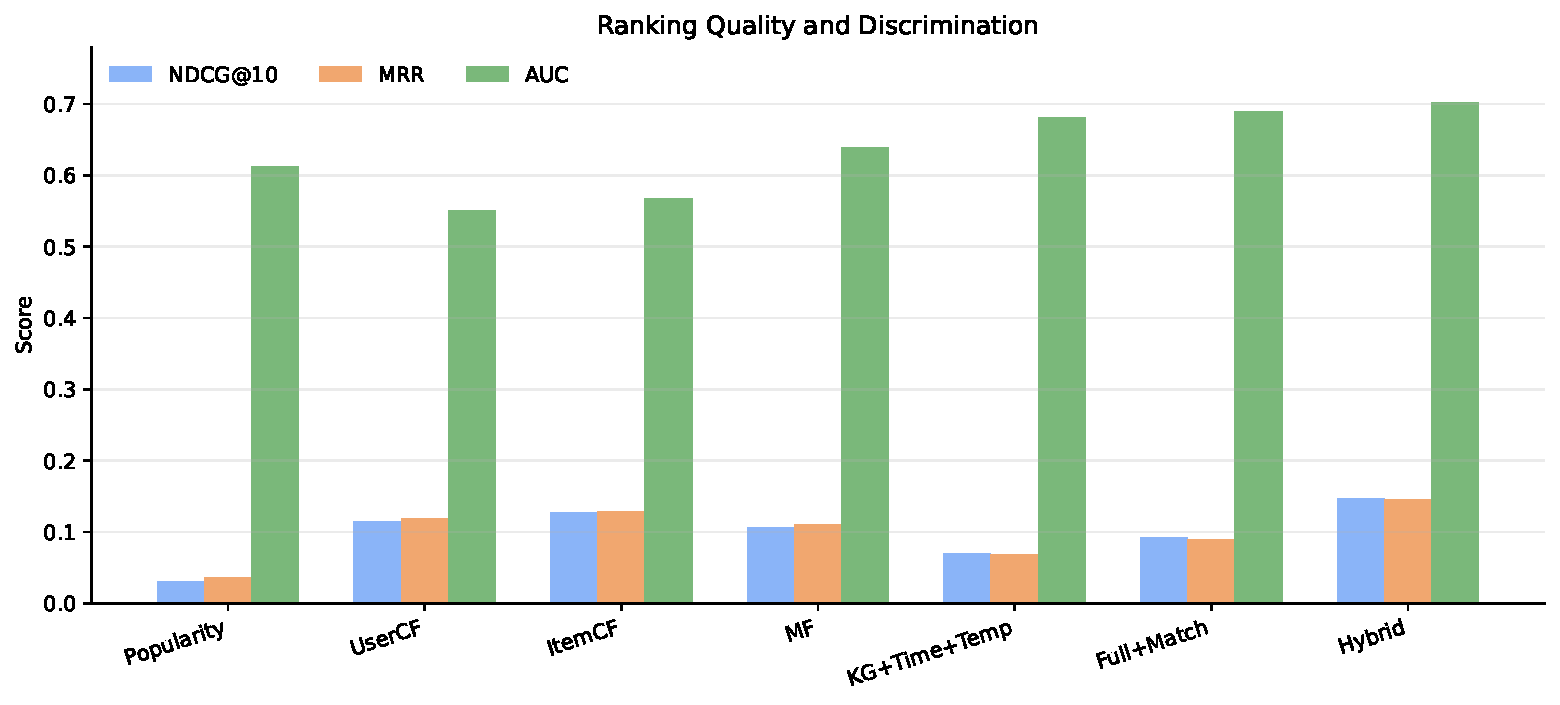
\includegraphics[width=0.96\linewidth]{figures/ranking_quality.pdf}
\caption{主要模型在 NDCG@10、MRR 和 AUC 上的对比}
\end{figure}

\begin{figure}[htbp]
\centering
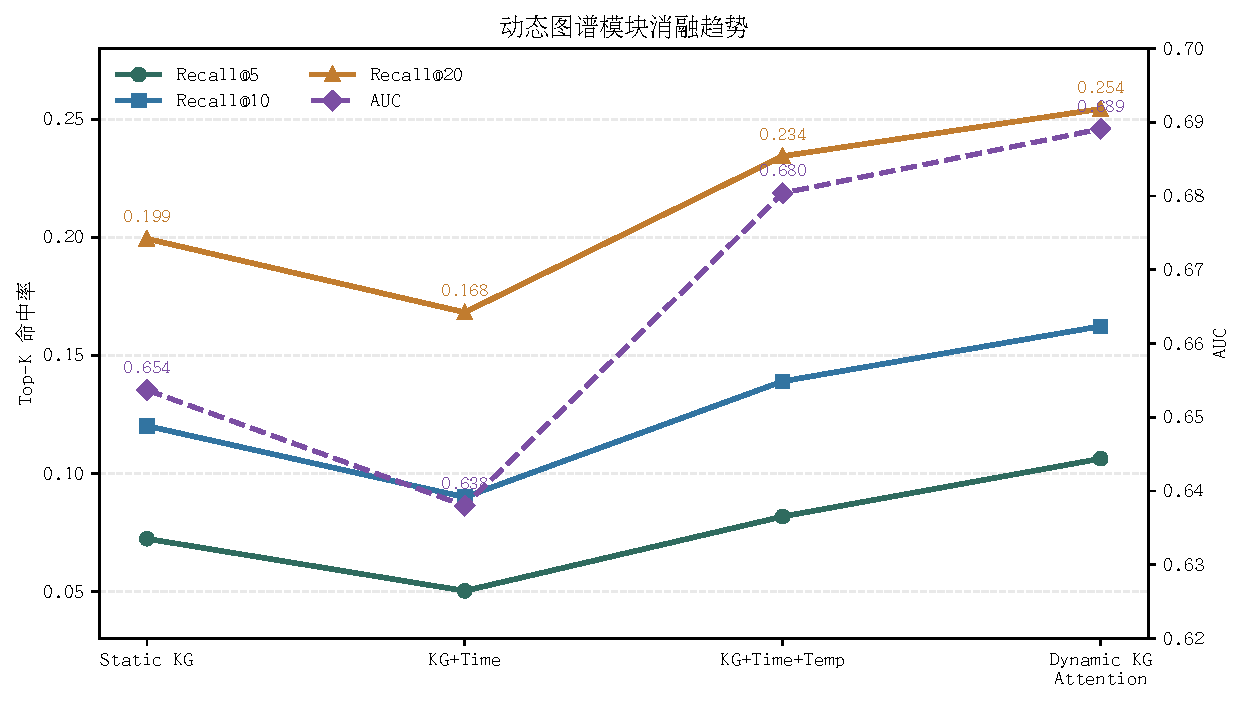
\includegraphics[width=0.92\linewidth]{figures/dynamic_ablation.pdf}
\caption{动态图谱模块消融趋势}
\end{figure}

\begin{figure}[htbp]
\centering
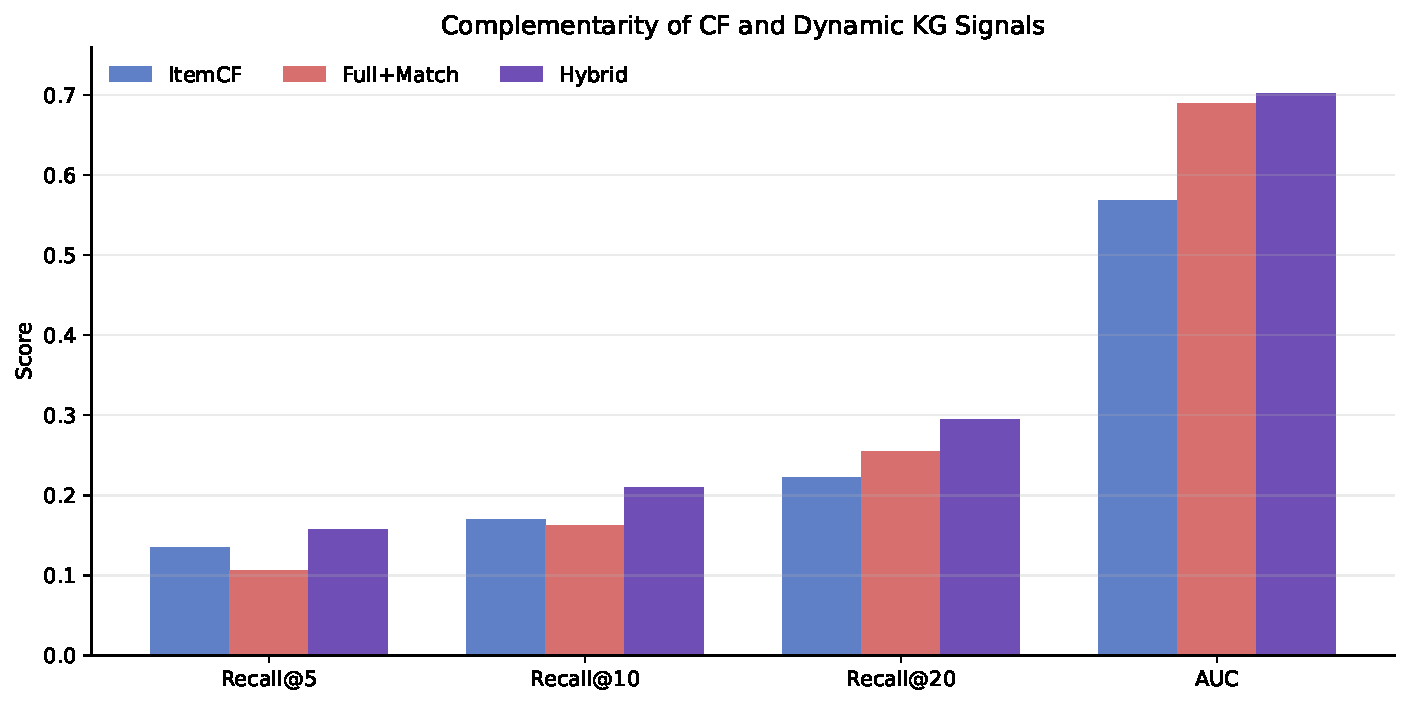
\includegraphics[width=0.88\linewidth]{figures/final_model_gain.pdf}
\caption{ItemCF、Dynamic KG Attention 与最终融合模型的互补效果}
\end{figure}

\begin{figure}[htbp]
\centering
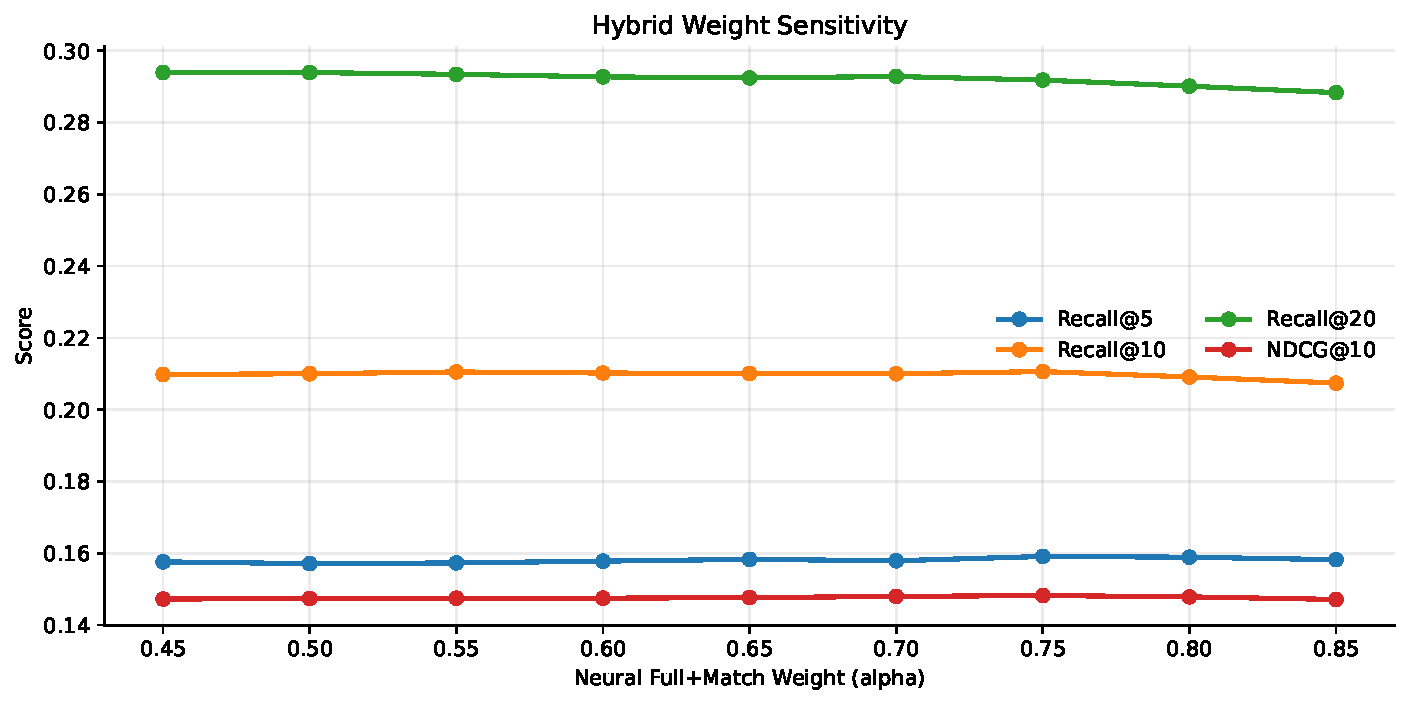
\includegraphics[width=0.88\linewidth]{figures/hybrid_weight_curve.pdf}
\caption{Final Hybrid 中神经模型权重对指标的影响}
\end{figure}

\begin{table}[htbp]
\centering
\caption{Final Hybrid 相对核心模型的指标提升（百分点）}
\small
\begin{tabular}{lrrrrr}
\toprule
对照模型 & Recall@5 & Recall@10 & Recall@20 & NDCG@10 & AUC \\
\midrule
ItemCF & +2.2 & +4.0 & +7.1 & +2.0 & +13.4\\
Static KG & +8.5 & +9.0 & +9.5 & +8.3 & +4.9\\
KG + Time + Temp & +7.6 & +7.1 & +6.0 & +7.7 & +2.2\\
Dynamic KG Attention & +5.1 & +4.8 & +4.0 & +5.5 & +1.3\\
\bottomrule
\end{tabular}
\end{table}

从表中可以看到，Popularity 表现较弱，说明在随机负候选条件下，仅依赖商家热度不足以完成个性化排序。UserCF 和 ItemCF 在头部命中指标上较强，说明外卖存在明显的重复消费和相似商家替代关系，纯协同过滤能够较好地抓住用户稳定偏好。MF 在 AUC 上优于协同过滤，但 Top-K 命中不如 ItemCF，说明 MF 的整体正负区分能力较好，但对最前几名排序的优化不足。

知识图谱模型中，Static KG 的 AUC 高于 MF，说明商家类目、口味、价格、评分、区域、菜品属性等结构化属性能改善整体区分能力。加入时间衰减和临时兴趣后，KG + Time + Temp 在 Recall@20 和 AUC 上超过 Static KG 与 KG + Time，表明下单前点击序列对较宽推荐列表和整体排序区分有增益。

Dynamic KG Attention 将候选商家属性与当前动态兴趣的重合程度显式加入排序特征，使动态图谱兴趣能够直接参与候选商家打分。Final Hybrid 将 ItemCF 的邻域协同信号与 Dynamic KG Attention 的图谱兴趣信号融合，在所有主指标上取得最佳结果：Recall@5、Recall@10、Recall@20 分别达到 0.157、0.210、0.294，AUC 达到 0.702。该结果说明协同过滤的局部邻域信号与动态图谱注意力模型的属性/兴趣信号具有明显互补性。

\section{可解释推荐示例}

模型可根据用户动态图谱兴趣和候选商家属性重合路径解释推荐。以下为 \path{outputs/explain\_gpu\_100k.txt} 中的真实输出节选：

\begin{quote}
用户 121762 的某次请求中，真实下单商家 2876 被排在第 1 位，解释路径包括：
\begin{itemize}
  \item 历史订单时间衰减兴趣 $\rightarrow$ \texttt{cat1:0} $\rightarrow$ 候选商家；
  \item 历史订单时间衰减兴趣 $\rightarrow$ \texttt{price:[49,65)} $\rightarrow$ 候选商家；
  \item 历史订单时间衰减兴趣 $\rightarrow$ \texttt{poi\_score:medium} $\rightarrow$ 候选商家；
  \item 历史订单时间衰减兴趣 $\rightarrow$ \texttt{delivery\_score:excellent} $\rightarrow$ 候选商家。
\end{itemize}
\end{quote}

这类解释可转化为业务文案，例如 ``你近期下单过相同大类、相近价格区间且配送评分较高的商家，因此该候选商家更符合当前偏好''。由于 TRD 对商家和菜品名称做了脱敏，本文解释以实体 ID 和属性类型展示；若换成未脱敏数据，可直接输出 ``川菜、麻辣、轻食、低价、某区域'' 等自然语言标签。

\section{核心代码框架}

项目核心代码如下：

\begin{itemize}
  \item \texttt{scripts/download\_trd.py}：从 Zenodo 下载 TRD 文本数据并做 MD5 校验。
  \item \texttt{src/prepare\_data.py}：清洗数据，构造静态知识图谱、历史时间衰减兴趣、点击临时兴趣、训练样本和测试候选集。
  \item \texttt{src/model.py}：实现 DynamicKGAttentionRecommender 和 MF。
  \item \texttt{src/run\_baselines.py}：实现 Popularity、UserCF、ItemCF。
  \item \texttt{src/run\_experiment.py}：训练和评价 MF、Static KG、KG + Time、KG + Time + Temp、Dynamic KG Attention。
  \item \texttt{src/explain\_recommend.py}：输出 Top-K 推荐及图谱路径解释。
\end{itemize}

动态图谱样本构造伪代码如下：

\begin{lstlisting}[language=Python,caption={动态兴趣构造伪代码}]
for order in user_orders_sorted_by_time:
    u, target_poi, T = order.user, order.poi, order.timestamp
    interest = Counter()

    for poi, t in recent_history[u]:
        decay = exp(-lambda_ * (T - t) / seconds_per_day)
        for entity in KG.neighbors(poi):
            interest[(entity, "pref_hist")] += decay

    clicks = pre_order_click_session[order.id][-max_clicks:]
    for pos, poi in enumerate(clicks):
        weight = click_weight * click_decay ** (len(clicks) - pos - 1)
        for entity in KG.neighbors(poi):
            interest[(entity, "pref_click")] += weight

    dynamic_neighbors = top_weighted_entities(interest, max_interests)
    train_pair = (u, target_poi, dynamic_neighbors, label=1)
    negative_pairs = sample_negative_pois(u)
\end{lstlisting}

关系感知注意力核心代码如下：

\begin{lstlisting}[language=Python,caption={关系感知动态注意力核心}]
logits = attn_vec(tanh(
    Wq(user_embedding).unsqueeze(1)
    + We(entity_embedding)
    + Wr(relation_embedding)
)).squeeze(-1)
logits = logits + log1p(dynamic_preference_weight)
alpha = masked_softmax(logits, interest_mask)
h_user = layer_norm(user_embedding + sum(alpha * (entity_embedding + relation_embedding)))
score = MLP(concat([h_user, h_poi, h_user * h_poi, basic_features]))
\end{lstlisting}

\section{创新点总结}

本文创新点围绕餐饮外卖场景展开：

\begin{enumerate}
  \item 构建餐饮外卖领域知识图谱，将商家、菜系/类目、口味、食材、价格区间、评分等级、区域、品牌、标准菜品等实体结构化。
  \item 将用户连续历史订单序列转化为动态图谱边权，通过指数时间衰减表达外卖偏好的时效性，而不是直接套用传统序列推荐模型。
  \item 利用下单前点击商家序列生成临时兴趣节点，表达用户 ``当前这一餐'' 的短期饮食偏好。
  \item 使用关系感知图注意力机制动态聚合历史偏好和点击临时偏好，区分 \texttt{pref\_hist}、\texttt{pref\_click} 以及不同商家属性关系。
  \item 排序阶段融合动态图谱用户表示、商家图谱表示和基础上下文特征，在准确性之外提供可解释推荐路径。
\end{enumerate}

\section{不足与改进方向}

本文实验仍有改进空间。第一，当前评价是 sampled ranking，每个测试查询只在 200 个候选商家内排序，尚未做到全量 29071 个商家检索；后续应增加召回阶段或采用分块全量打分，报告 full-catalog Recall@K。第二，神经模型采用 pointwise BCE 损失，后续可改用 BPR、softmax cross-entropy、LambdaRank 等 pairwise/listwise 目标进一步优化头部排序。第三，当前负样本主要按热度分布采样，尚未显式构造同区域、同餐段、同价格区间、同菜系的困难负样本。第四，TRD 名称字段经过脱敏，解释路径目前以属性 ID 展示，自然语言可读性受限。第五，可进一步加入完整 LightGCN、KGAT、DeepFM 或 LightGBM 排序层，与本文动态图谱兴趣模块做融合比较。

\begin{thebibliography}{99}
\bibitem{trd2023}
Yijian Liu. Takeout Recommendation Dataset (TRD) from Meituan Takeout app. Zenodo, 2023. DOI: \href{https://doi.org/10.5281/zenodo.8025855}{10.5281/zenodo.8025855}.

\bibitem{meituan_kg_blog}
美团技术团队. 美团外卖美食知识图谱的迭代及应用. 2021. \url{https://tech.meituan.com/2021/05/27/Food-Knowledge-Graph.html}.

\bibitem{kgat}
Xiang Wang, Xiangnan He, Yixin Cao, Meng Liu, Tat-Seng Chua. KGAT: Knowledge Graph Attention Network for Recommendation. KDD 2019. \url{https://arxiv.org/abs/1905.07854}.

\bibitem{lightgcn}
Xiangnan He, Kuan Deng, Xiang Wang, Yan Li, Yongdong Zhang, Meng Wang. LightGCN: Simplifying and Powering Graph Convolution Network for Recommendation. SIGIR 2020. \url{https://arxiv.org/abs/2002.02126}.

\bibitem{deepfm}
Huifeng Guo, Ruiming Tang, Yunming Ye, Zhenguo Li, Xiuqiang He. DeepFM: A Factorization-Machine based Neural Network for CTR Prediction. IJCAI 2017. \url{https://arxiv.org/abs/1703.04247}.
\end{thebibliography}

\end{document}
